

%% CAP High School Prize Examination
%%----------------------------------------


%% this section contains 40 problems


%% CAP Exam 2015
%%----------------------------------------


%% CAP Exam 2014
%%----------------------------------------
\element{cap}{ %% cap-D1
\begin{question}{CAP-A-2014-q07}
    Three ping-pong balls are electrically charged and are arranged in the plane of the page in an equilateral triangle as shown below. 
    \begin{center}
    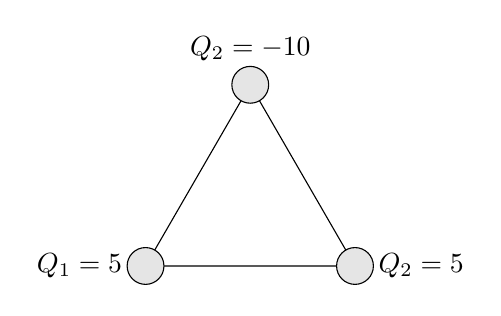
\begin{tikzpicture}[scale=1.33]
        \draw (0,0) -- (1,1.73) -- (2,0) -- cycle;
        \draw[fill=white!90!black] (0,0) circle (5pt) node[anchor=east,xshift=-5pt] {$Q_1=\SI{5}{\micro\coulomb}$};
        \draw[fill=white!90!black] (1,1.73) circle (5pt) node[anchor=south,yshift=5pt] {$Q_2=\SI{-10}{\micro\coulomb}$};
        \draw[fill=white!90!black] (2,0) circle (5pt) node[anchor=west,xshift=5pt] {$Q_2=\SI{5}{\micro\coulomb}$};
    \end{tikzpicture}
    \end{center}
    What is the direction of the force acting on the ping-pong ball charged with $Q_3 = \SI{-10}{\micro\coulomb}$?
    \begin{choices}
        \wrongchoice{Towards the top of the page.}
      \correctchoice{Towards the bottom of the page.}
        \wrongchoice{Towards the left.}
        \wrongchoice{Towards the right.}
        \wrongchoice{Another direction.}
    \end{choices}
\end{question}
}


%% CAP Exam 2013
%%----------------------------------------
\element{cap}{ %% cap-D1
\begin{question}{CAP-A-2013-q02}
    Consider the electric charges $A$, $B$, $C$ shown in the figure below,
        where $q$ is a positive number. 
    \begin{center}
    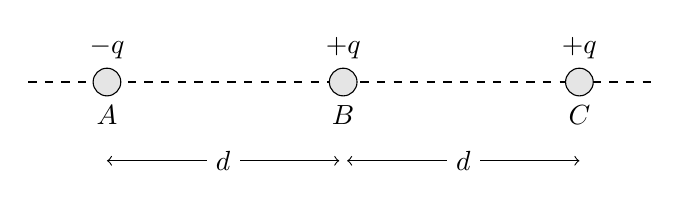
\begin{tikzpicture}
        %% axis
        \draw[dashed] (-4,0) -- (4,0);
        %% charges
        \draw[fill=white!90!black] (-3,0) circle (5pt)
            node[anchor=south,yshift=+5pt] {$-q$}
            node[anchor=north,yshift=-5pt] {$A$};
        \draw[fill=white!90!black] (0,0) circle (5pt)
            node[anchor=south,yshift=+5pt] {$+q$}
            node[anchor=north,yshift=-5pt] {$B$};
        \draw[fill=white!90!black] (3,0) circle (5pt)
            node[anchor=south,yshift=+5pt] {$+q$}
            node[anchor=north,yshift=-5pt] {$C$};
        %% distances
        \draw[<->] (-3,-1) -- (-0.05,-1) node[pos=0.5,anchor=center,fill=white] {$d$};
        \draw[<->] (+3,-1) -- (+0.05,-1) node[pos=0.5,anchor=center,fill=white] {$d$};
    \end{tikzpicture}
    \end{center}
    Which answer correctly describes the magnitude of the net force experienced by the charges?
    \begin{multicols}{2}
    \begin{choices}
        \wrongchoice{$F_A > F_B > F_C$}
        \wrongchoice{$F_A > F_C > F_B$}
      \correctchoice{$F_B > F_A > F_C$}
        \wrongchoice{$F_A = F_B = F_C$}
        \wrongchoice{$F_A > F_B = F_C$}
    \end{choices}
    \end{multicols}
\end{question}
}

\element{cap}{ %% cap-D1
\begin{question}{CAP-A-2013-q11}
    Two point charges $-2Q$ and $+Q$ are placed on the $x$-axis with $-2Q$ at $x=0$ and $+Q$ at $x=a$.
    Which of the following statements is true?
    \begin{choices}
        \wrongchoice{There is no point on the $x$-axis where the electric field is zero.}
        \wrongchoice{There is a point on the $x$-axis, at $x<0$, where the electric field is zero.}
        \wrongchoice{There is a point on the $x$-axis, between the charges ($0<x<a$), where the electric field is zero.}
      \correctchoice{There is a point on the $x$-axis, at $x>a$, where the electric field is zero.}
    \end{choices}
\end{question}
}


%% CAP Exam 2010
%%----------------------------------------
\element{cap}{ %% cap-D1
\begin{question}{CAP-A-2010-q14}
    Eight identical negative charges $-q$ are arranged symmetrically on a circle of radius $r$,
        each equidistant from the next. 
    \begin{center}
    \begin{tikzpicture}
        \draw (0,0) circle (2cm);
        \foreach \x in {45,90,...,360} {
            \draw[fill] (\x:2) circle (1.5pt) node[anchor=center,shift={(\x:1em)}] {$-q$};
        }
    \end{tikzpicture}
    \end{center}
    Assume the point charges have zero potential at infinity. 
    If the constant of proportionality in Coulomb's law is $k$,
        then the magnitude of the electric field and the electrostatic potential at the center of the circle are given by:
    \begin{choices}
        \wrongchoice{$E=\dfrac{8kq}{r^2}$; $V=\dfrac{-8kq}{r}$}
        \wrongchoice{$E=\dfrac{8kq}{\left(2\pi r\right)^2}$; $V=\dfrac{-8kq}{2\pi r}$}
        \wrongchoice{$E=\dfrac{8kq}{r^2}$; $V=0$}
        \wrongchoice{$E=0$; $V=0$}
      \correctchoice{$E=0$; $V=\dfrac{-8kq}{r}$}
    \end{choices}
\end{question}
}

\element{cap}{ %% cap-D1
\begin{question}{CAP-A-2010-q15}
    %% NOTE: made independnet
    Five negative charges $-q$ and three positive charges $+q$
        all of the same magnitude are arranged symmetrically on a circle of radius $r$,
        each equidistant from the next. 
    \begin{center}
    \begin{tikzpicture}
        \draw (0,0) circle (2cm);
        \foreach \x in {90,125,...,270} {
            \draw[fill] (\x:2) circle (1.5pt) node[anchor=center,shift={(\x:1em)}] {$-q$};
        }
        \foreach \x in {315,360,45} {
            \draw[fill] (\x:2) circle (1.5pt) node[anchor=center,shift={(\x:1em)}] {$+q$};
        }
    \end{tikzpicture}
    \end{center}
    %Three of the negative charges in the previous questions are replaced with positive charges with the same magnitude,
    %    and are arranged as in the figure.
    %The magnitude of the electric field and the electrostatic potential at the center of the circle are given by:
    Assume the point charges have zero potential at infinity. 
    If the constant of proportionality in Coulomb's law is $k$,
        then the magnitude of the electric field and the electrostatic potential at the center of the circle are given by:
    \begin{choices}
        \wrongchoice{$E=\dfrac{2kq}{r^2}\left(1+2\sqrt{2}\right)$; $V=0$}
      \correctchoice{$E=\dfrac{2kq}{r^2}\left(1+\sqrt{2}\right)$; $V=\dfrac{-2kq}{r}$}
        \wrongchoice{$E=\dfrac{2kq}{r^2}\left(1+2\sqrt{2}\right)$; $V=\dfrac{-2kq}{r}$}
        \wrongchoice{$E=0$; $V=\dfrac{-2qk}{r}$}
        \wrongchoice{none of the provided}
    \end{choices}
\end{question}
}


\endinput


